\documentclass[11pt]{article}
\usepackage[textwidth=18.0cm, textheight=23.0cm, top=2.0cm]{geometry}
\usepackage{pst-all}
\usepackage{amssymb}
\usepackage{tikz}
\usepackage{underscore}\begin{document}
\pagestyle{empty}


ClassName: \underline{\textbf{Class_10.2bp-22}}
\par
BinSize: \underline{\textbf{100 × 100}}
\par
ReduceSize: \underline{\textbf{100 × 100}}
\par
TypeNum: \underline{\textbf{60}}
\par
Num: \underline{\textbf{60}}
\par
OutS: \underline{\textbf{110000}}
\par
InS: \underline{\textbf{102593}}
\par
Rate: \underline{\textbf{0.933}}
\par
UB: \underline{\textbf{11}}
\par
LB0: \underline{\textbf{11}}
\par
LB: \underline{\textbf{11}}
\par
LBWithCut: \underline{\textbf{11}}
\par
NodeCut: \underline{\textbf{0}}
\par
ExtendedNodeCnt: \underline{\textbf{1}}
\par
GenNodeCnt: \underline{\textbf{1}}
\par
PrimalNode: \underline{\textbf{0}}
\par
ColumnCount: \underline{\textbf{11}}
\par
TotalCutCount: \underline{\textbf{0}}
\par
RootCutCount: \underline{\textbf{0}}
\par
LPSolverCnt: \underline{\textbf{1}}
\par
PricingSolverCnt: \underline{\textbf{0}}
\par
BranchAndBoundNum: \underline{\textbf{1}}
\par
isOpt: \underline{\textbf{true}}
\par
TimeOnPrimal: \underline{\textbf{0.000 s}}
\par
TimeOnPricing: \underline{\textbf{0.000 s}}
\par
TimeOnRmp: \underline{\textbf{0.063 s}}
\par
TotalTime: \underline{\textbf{0.125 s}}
\par
\newpage


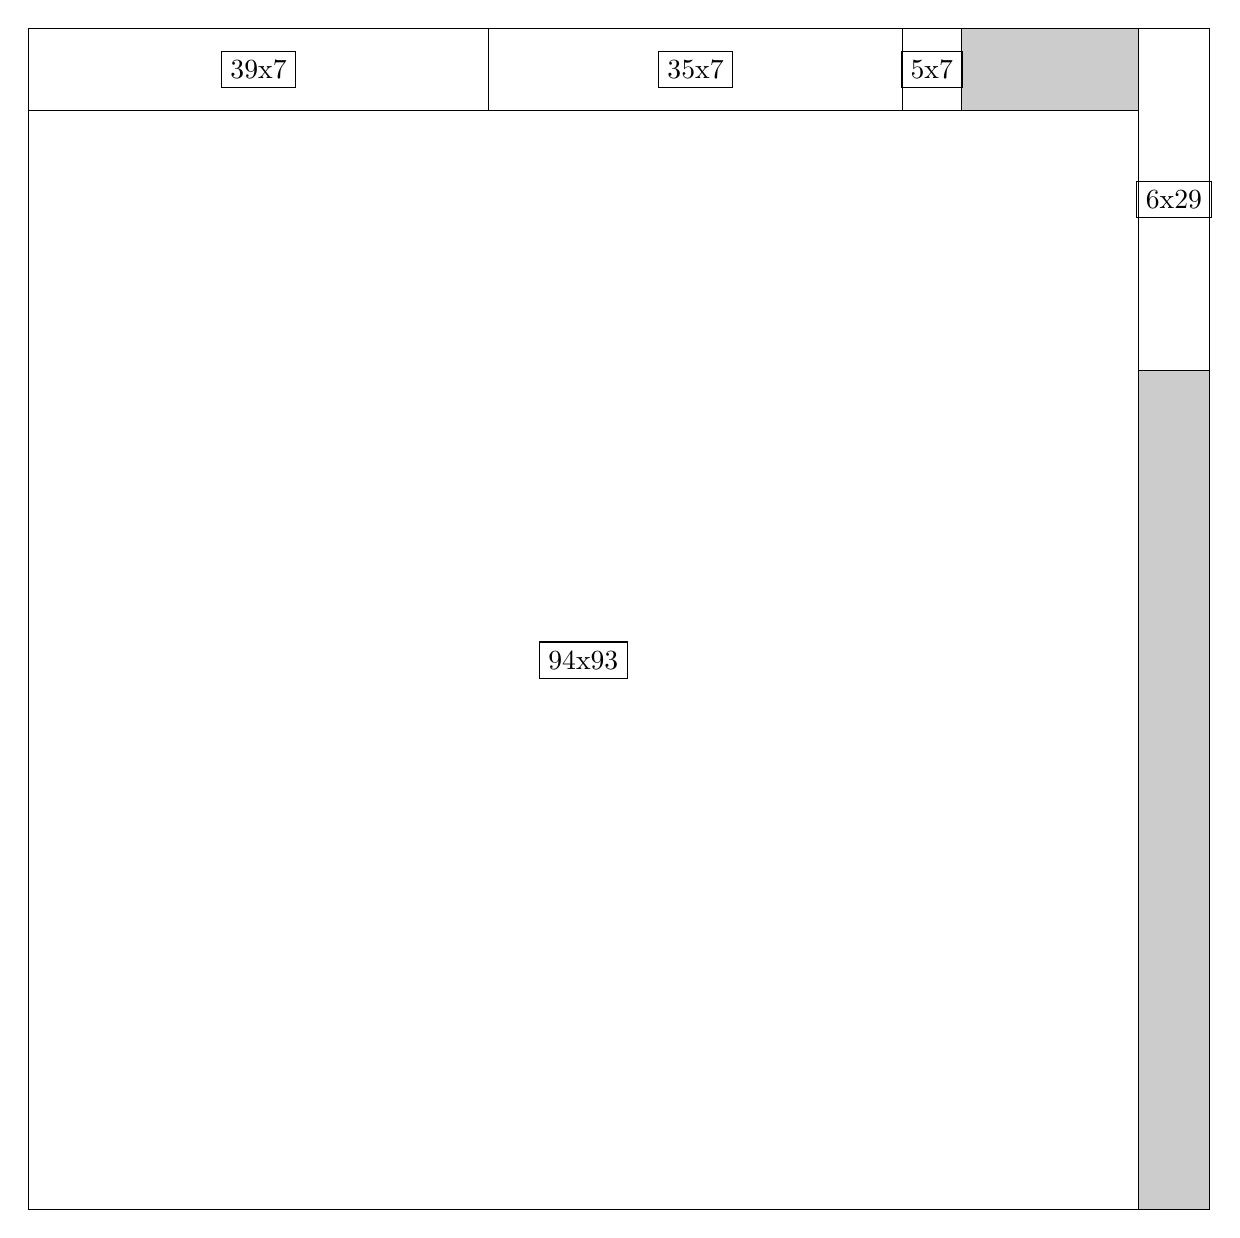
\begin{tikzpicture}[shorten >=1pt,scale=1.0,every node/.style={scale=1.0},->]
\tikzstyle{vertex}=[circle,fill=black!25,minimum size=14pt,inner sep=0pt]
\filldraw[fill=gray!40!white, draw=black] (0,0) rectangle (15.0,15.0);
\foreach \name/\x/\y/\w/\h in {94x93/0.0/0.0/14.1/13.95,39x7/0.0/13.95/5.85/1.05,35x7/5.85/13.95/5.25/1.05,6x29/14.1/10.65/0.8999999999999999/4.35,5x7/11.1/13.95/0.75/1.05}
\filldraw[fill=white!40!white, draw=black] (\x,\y) rectangle node[draw] (\name) {\name} ++(\w,\h);
\end{tikzpicture}


w =94 , h =93 , x =0 , y =0 , v =8742
\par
w =39 , h =7 , x =0 , y =93 , v =273
\par
w =35 , h =7 , x =39 , y =93 , v =245
\par
w =6 , h =29 , x =94 , y =71 , v =174
\par
w =5 , h =7 , x =74 , y =93 , v =35
\par
\newpage


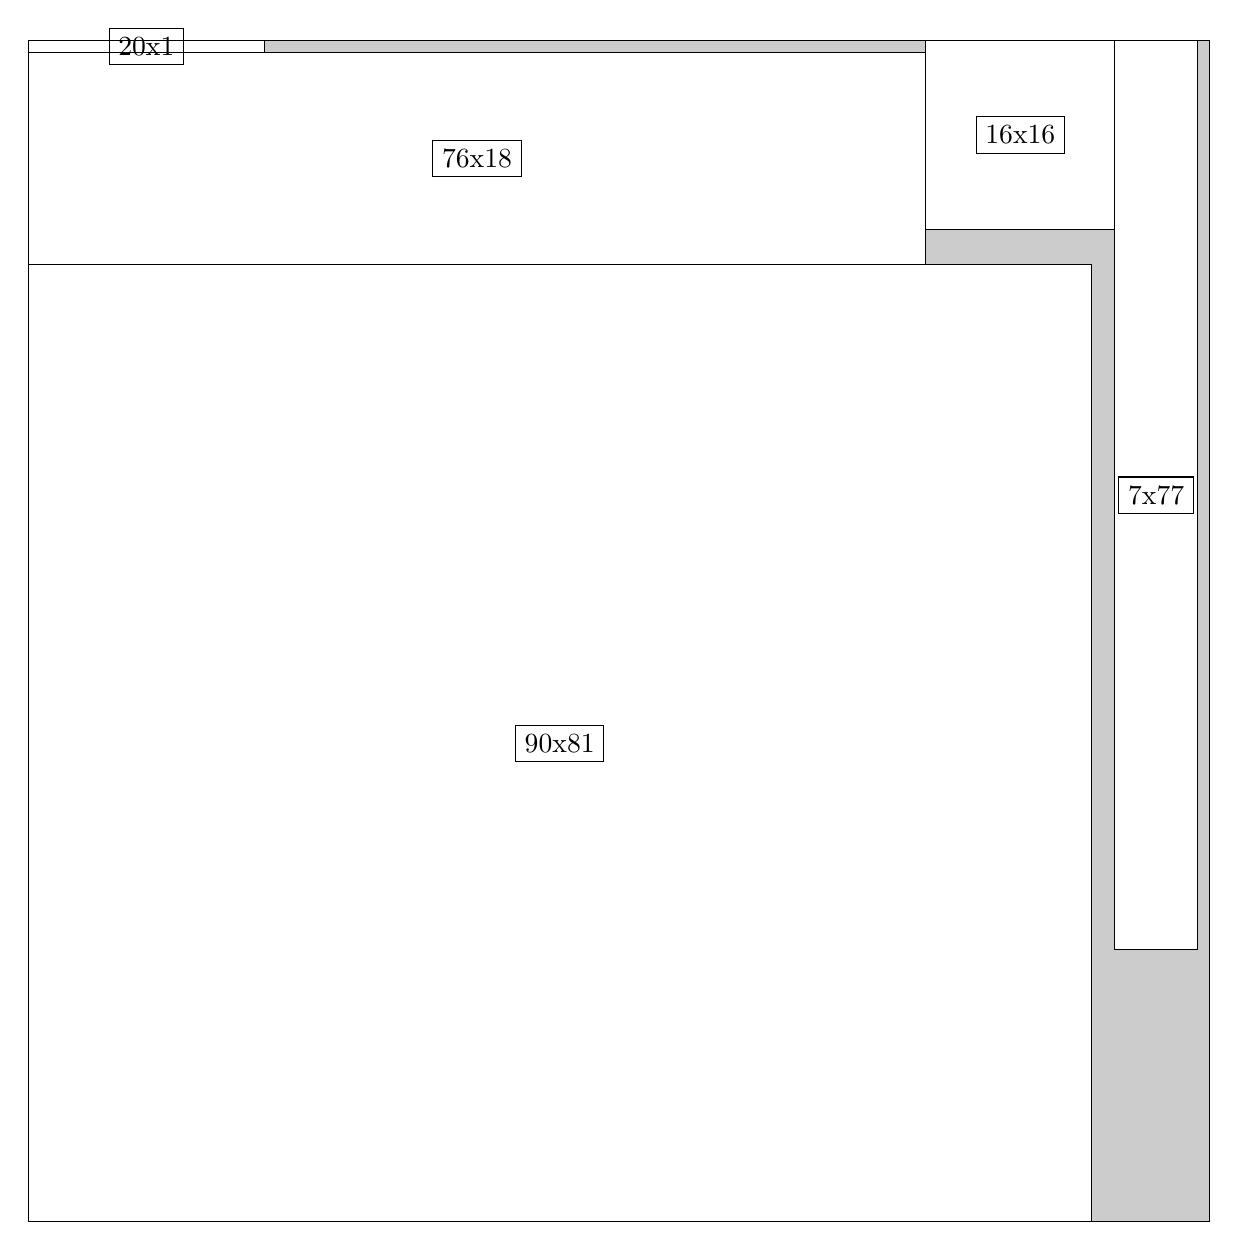
\begin{tikzpicture}[shorten >=1pt,scale=1.0,every node/.style={scale=1.0},->]
\tikzstyle{vertex}=[circle,fill=black!25,minimum size=14pt,inner sep=0pt]
\filldraw[fill=gray!40!white, draw=black] (0,0) rectangle (15.0,15.0);
\foreach \name/\x/\y/\w/\h in {90x81/0.0/0.0/13.5/12.15,76x18/0.0/12.15/11.4/2.6999999999999997,7x77/13.799999999999999/3.4499999999999997/1.05/11.549999999999999,16x16/11.4/12.6/2.4/2.4,20x1/0.0/14.85/3.0/0.15}
\filldraw[fill=white!40!white, draw=black] (\x,\y) rectangle node[draw] (\name) {\name} ++(\w,\h);
\end{tikzpicture}


w =90 , h =81 , x =0 , y =0 , v =7290
\par
w =76 , h =18 , x =0 , y =81 , v =1368
\par
w =7 , h =77 , x =92 , y =23 , v =539
\par
w =16 , h =16 , x =76 , y =84 , v =256
\par
w =20 , h =1 , x =0 , y =99 , v =20
\par
\newpage


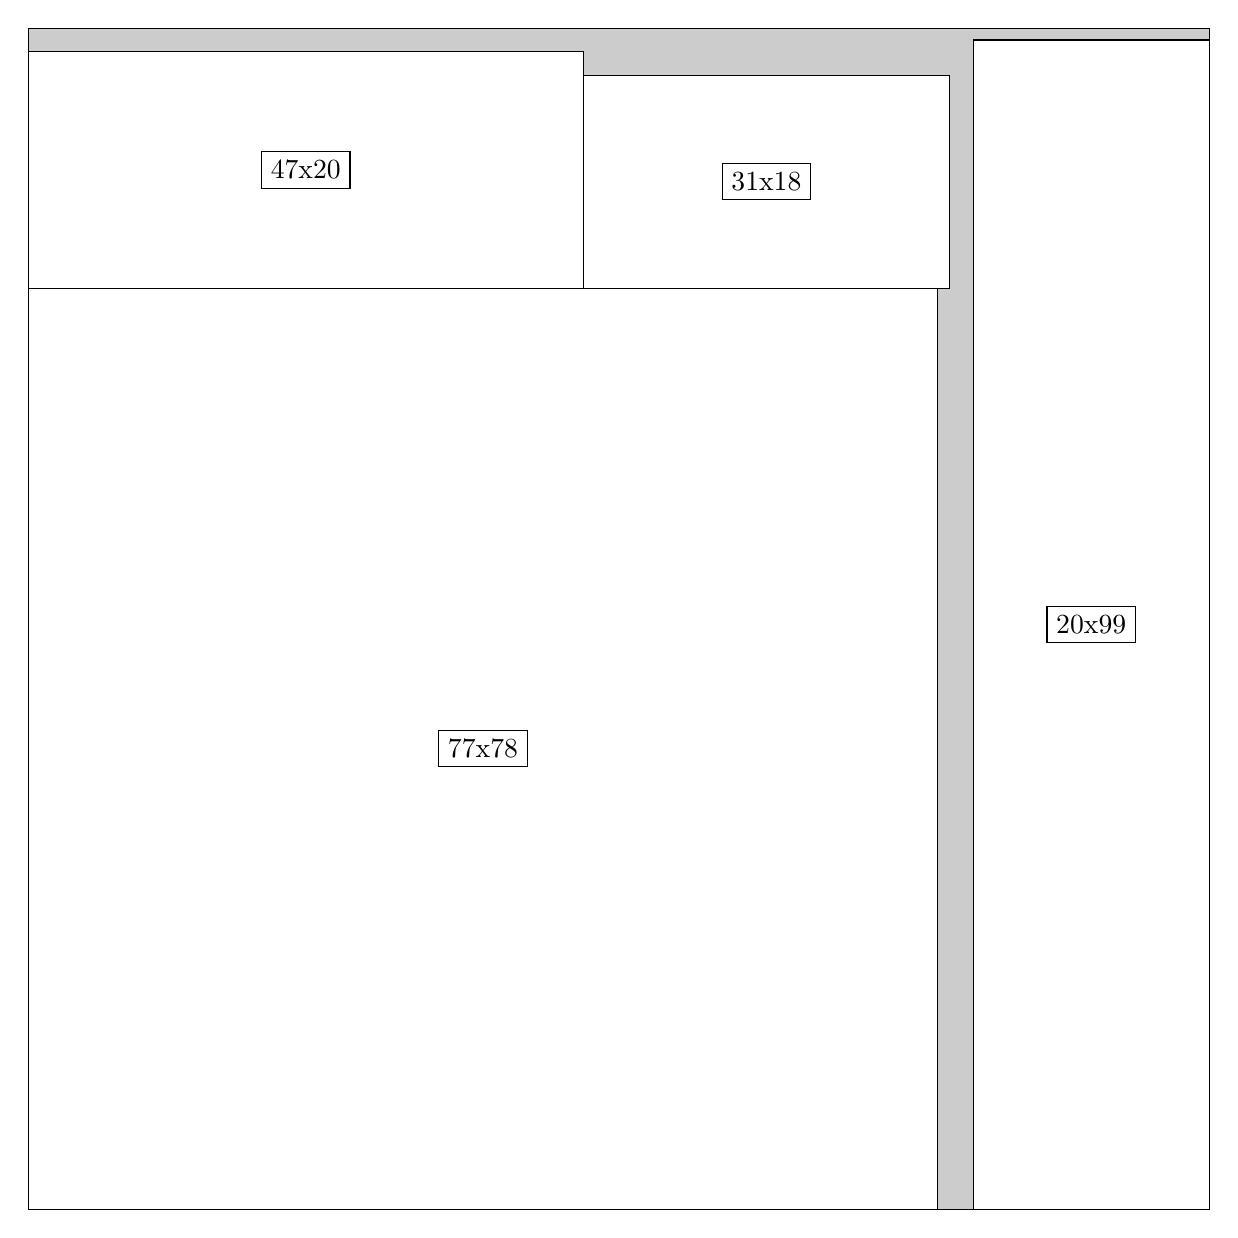
\begin{tikzpicture}[shorten >=1pt,scale=1.0,every node/.style={scale=1.0},->]
\tikzstyle{vertex}=[circle,fill=black!25,minimum size=14pt,inner sep=0pt]
\filldraw[fill=gray!40!white, draw=black] (0,0) rectangle (15.0,15.0);
\foreach \name/\x/\y/\w/\h in {77x78/0.0/0.0/11.549999999999999/11.7,20x99/12.0/0.0/3.0/14.85,47x20/0.0/11.7/7.05/3.0,31x18/7.05/11.7/4.6499999999999995/2.6999999999999997}
\filldraw[fill=white!40!white, draw=black] (\x,\y) rectangle node[draw] (\name) {\name} ++(\w,\h);
\end{tikzpicture}


w =77 , h =78 , x =0 , y =0 , v =6006
\par
w =20 , h =99 , x =80 , y =0 , v =1980
\par
w =47 , h =20 , x =0 , y =78 , v =940
\par
w =31 , h =18 , x =47 , y =78 , v =558
\par
\newpage


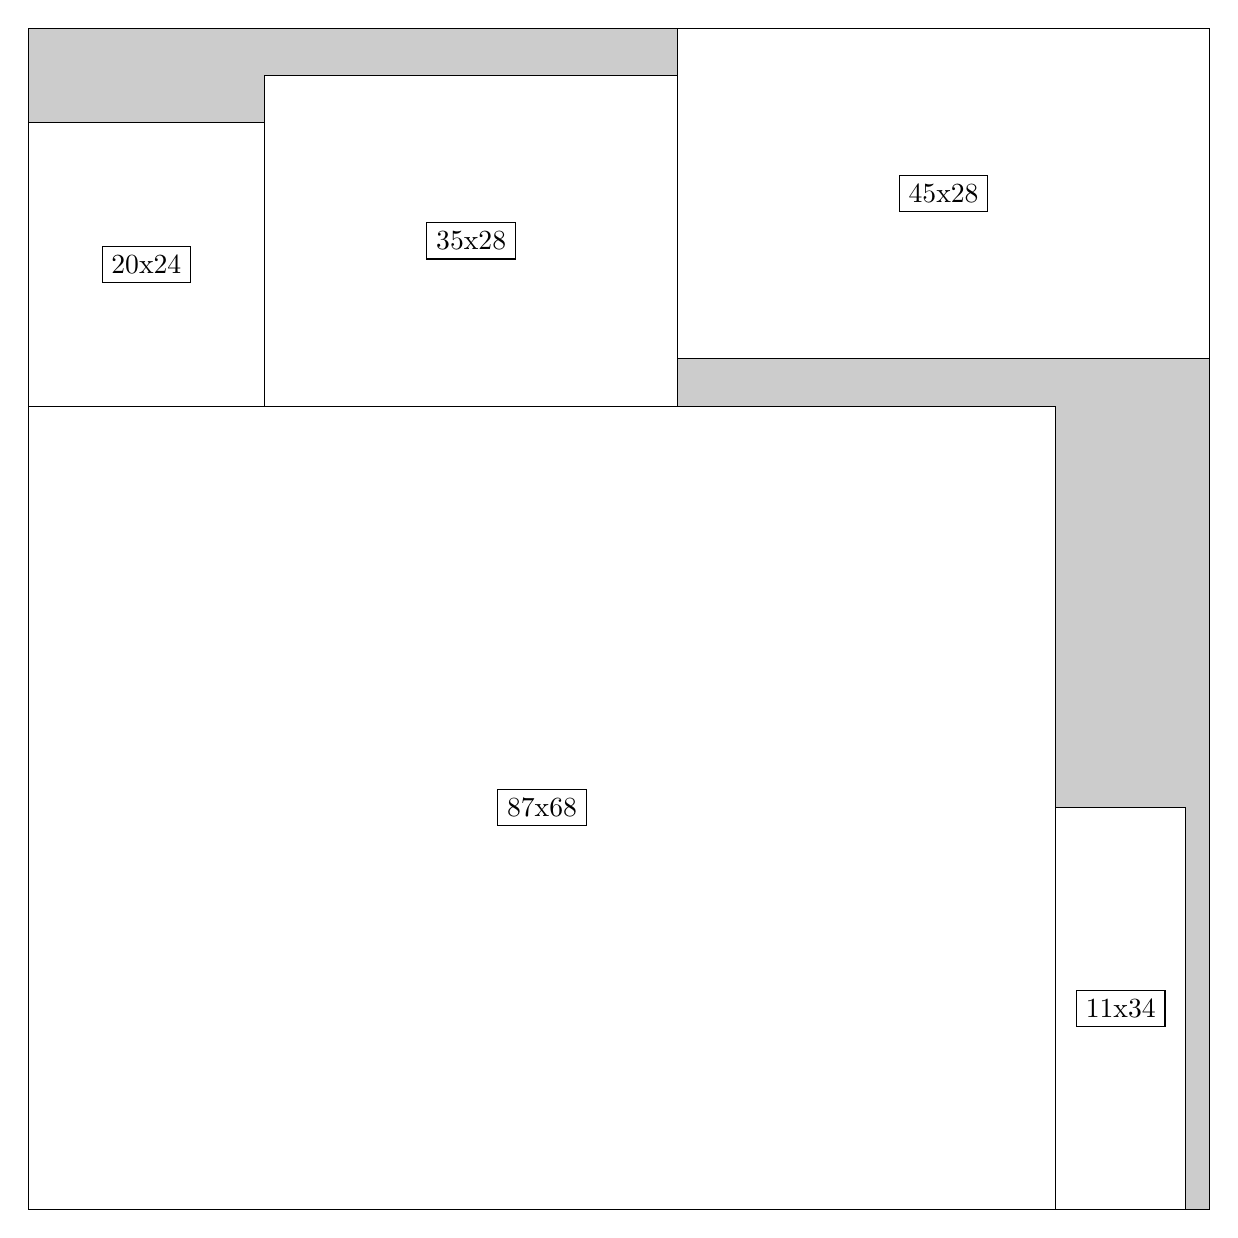
\begin{tikzpicture}[shorten >=1pt,scale=1.0,every node/.style={scale=1.0},->]
\tikzstyle{vertex}=[circle,fill=black!25,minimum size=14pt,inner sep=0pt]
\filldraw[fill=gray!40!white, draw=black] (0,0) rectangle (15.0,15.0);
\foreach \name/\x/\y/\w/\h in {20x24/0.0/10.2/3.0/3.5999999999999996,87x68/0.0/0.0/13.049999999999999/10.2,35x28/3.0/10.2/5.25/4.2,45x28/8.25/10.799999999999999/6.75/4.2,11x34/13.049999999999999/0.0/1.65/5.1}
\filldraw[fill=white!40!white, draw=black] (\x,\y) rectangle node[draw] (\name) {\name} ++(\w,\h);
\end{tikzpicture}


w =20 , h =24 , x =0 , y =68 , v =480
\par
w =87 , h =68 , x =0 , y =0 , v =5916
\par
w =35 , h =28 , x =20 , y =68 , v =980
\par
w =45 , h =28 , x =55 , y =72 , v =1260
\par
w =11 , h =34 , x =87 , y =0 , v =374
\par
\newpage


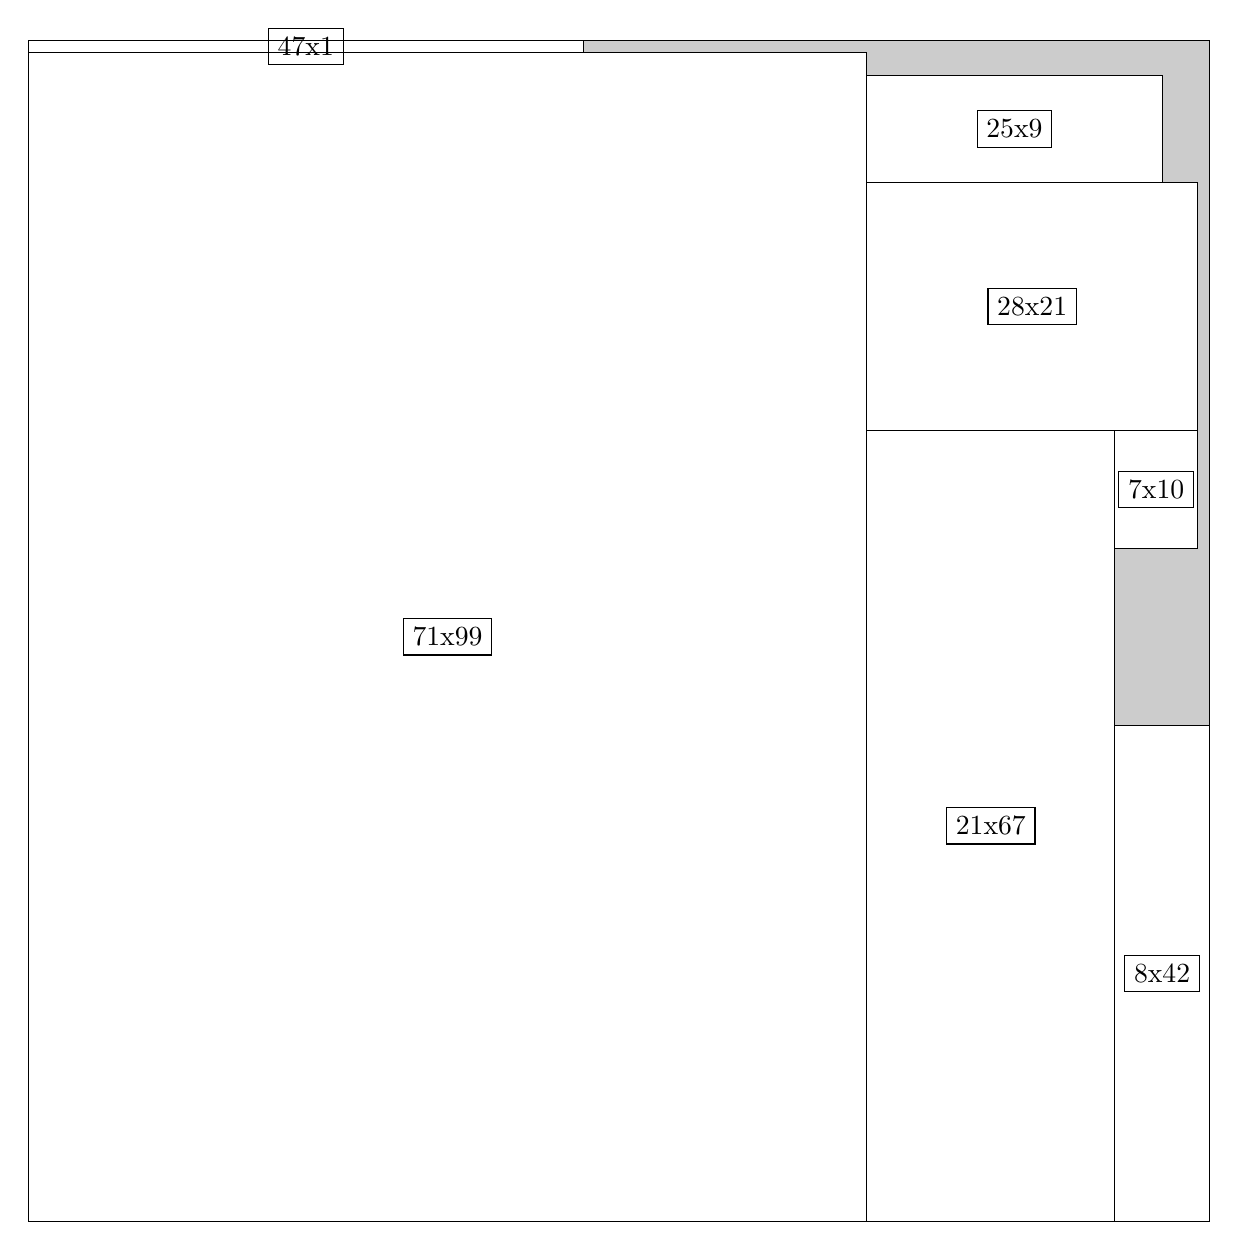
\begin{tikzpicture}[shorten >=1pt,scale=1.0,every node/.style={scale=1.0},->]
\tikzstyle{vertex}=[circle,fill=black!25,minimum size=14pt,inner sep=0pt]
\filldraw[fill=gray!40!white, draw=black] (0,0) rectangle (15.0,15.0);
\foreach \name/\x/\y/\w/\h in {71x99/0.0/0.0/10.65/14.85,21x67/10.65/0.0/3.15/10.049999999999999,28x21/10.65/10.049999999999999/4.2/3.15,8x42/13.799999999999999/0.0/1.2/6.3,25x9/10.65/13.2/3.75/1.3499999999999999,7x10/13.799999999999999/8.549999999999999/1.05/1.5,47x1/0.0/14.85/7.05/0.15}
\filldraw[fill=white!40!white, draw=black] (\x,\y) rectangle node[draw] (\name) {\name} ++(\w,\h);
\end{tikzpicture}


w =71 , h =99 , x =0 , y =0 , v =7029
\par
w =21 , h =67 , x =71 , y =0 , v =1407
\par
w =28 , h =21 , x =71 , y =67 , v =588
\par
w =8 , h =42 , x =92 , y =0 , v =336
\par
w =25 , h =9 , x =71 , y =88 , v =225
\par
w =7 , h =10 , x =92 , y =57 , v =70
\par
w =47 , h =1 , x =0 , y =99 , v =47
\par
\newpage


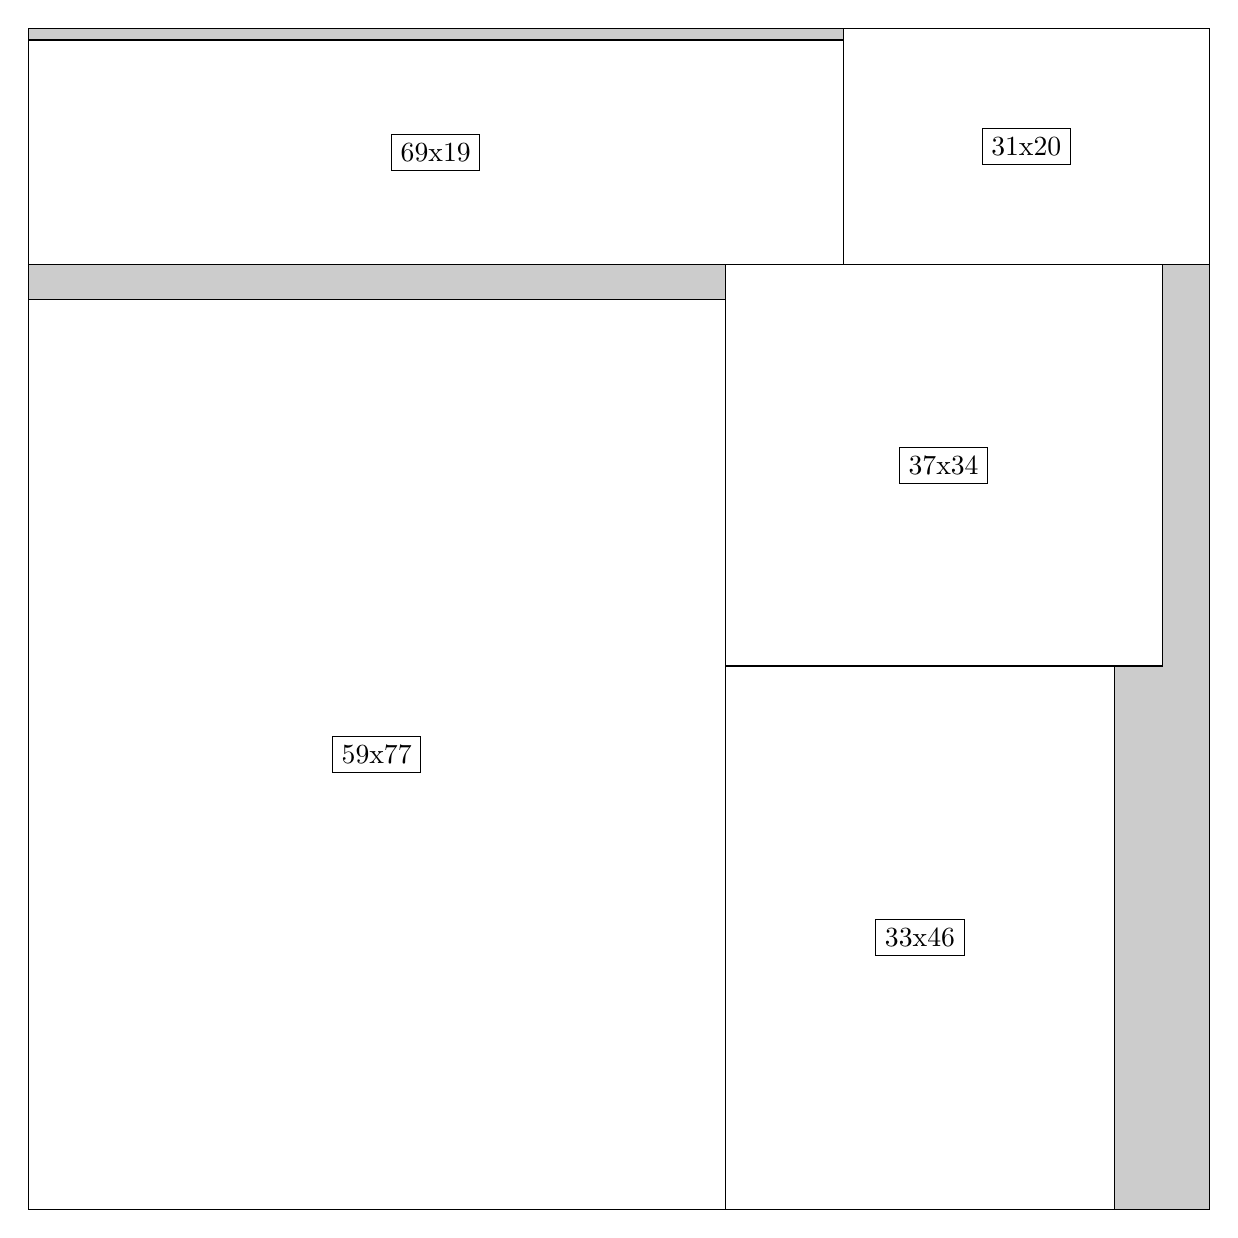
\begin{tikzpicture}[shorten >=1pt,scale=1.0,every node/.style={scale=1.0},->]
\tikzstyle{vertex}=[circle,fill=black!25,minimum size=14pt,inner sep=0pt]
\filldraw[fill=gray!40!white, draw=black] (0,0) rectangle (15.0,15.0);
\foreach \name/\x/\y/\w/\h in {59x77/0.0/0.0/8.85/11.549999999999999,33x46/8.85/0.0/4.95/6.8999999999999995,37x34/8.85/6.8999999999999995/5.55/5.1,31x20/10.35/12.0/4.6499999999999995/3.0,69x19/0.0/12.0/10.35/2.85}
\filldraw[fill=white!40!white, draw=black] (\x,\y) rectangle node[draw] (\name) {\name} ++(\w,\h);
\end{tikzpicture}


w =59 , h =77 , x =0 , y =0 , v =4543
\par
w =33 , h =46 , x =59 , y =0 , v =1518
\par
w =37 , h =34 , x =59 , y =46 , v =1258
\par
w =31 , h =20 , x =69 , y =80 , v =620
\par
w =69 , h =19 , x =0 , y =80 , v =1311
\par
\newpage


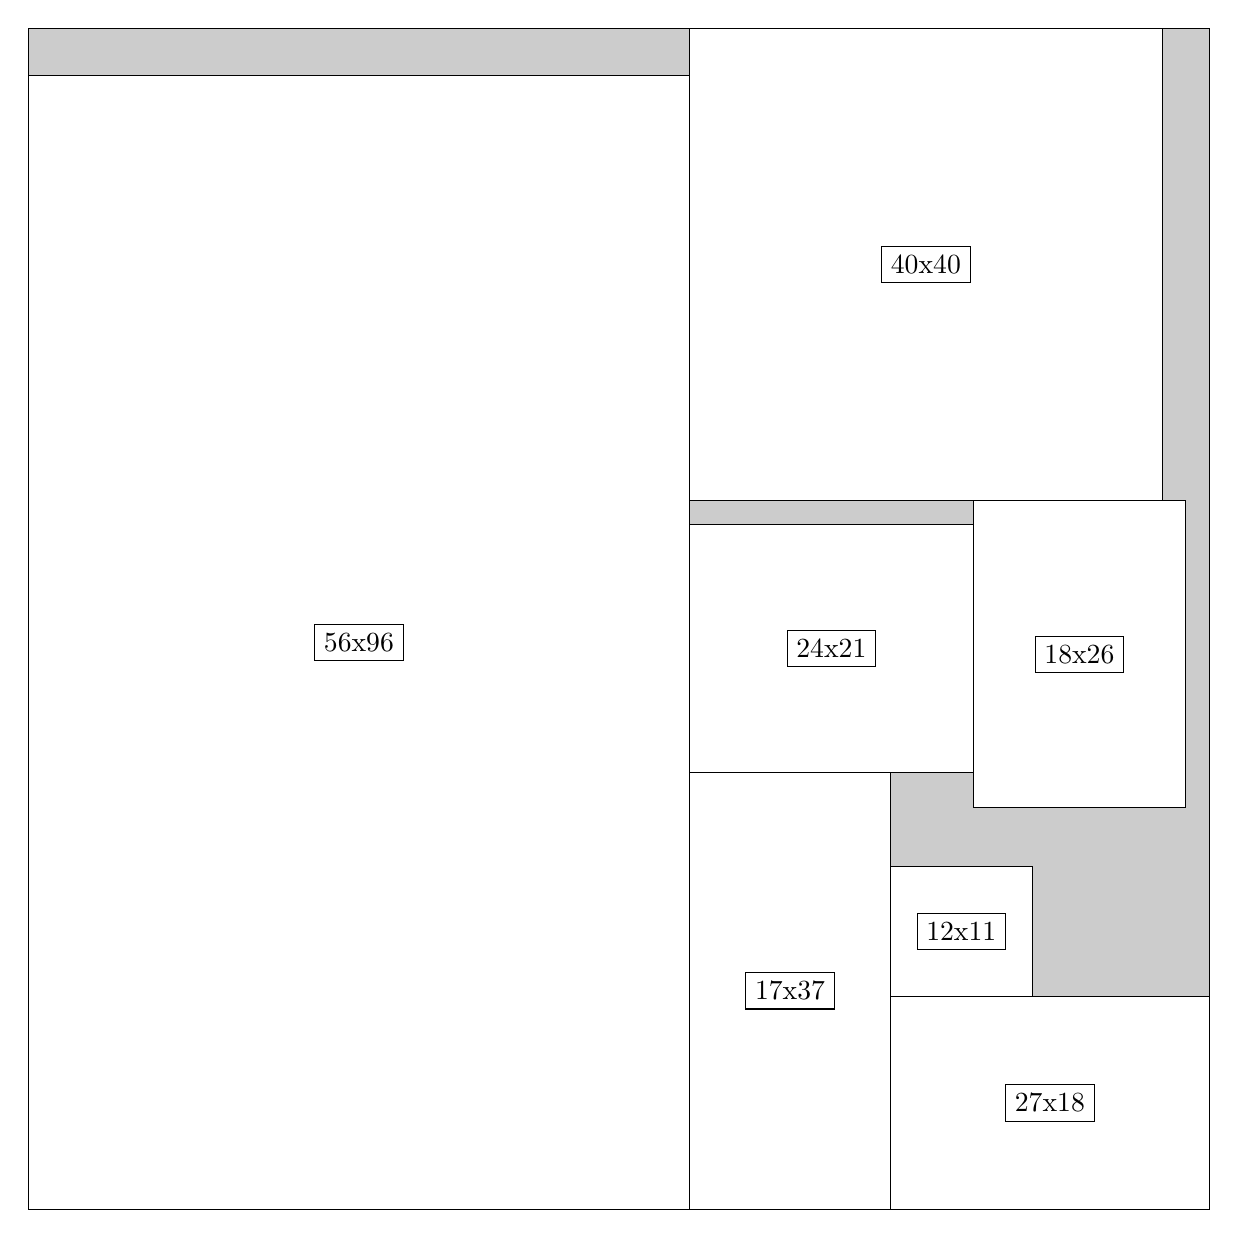
\begin{tikzpicture}[shorten >=1pt,scale=1.0,every node/.style={scale=1.0},->]
\tikzstyle{vertex}=[circle,fill=black!25,minimum size=14pt,inner sep=0pt]
\filldraw[fill=gray!40!white, draw=black] (0,0) rectangle (15.0,15.0);
\foreach \name/\x/\y/\w/\h in {56x96/0.0/0.0/8.4/14.399999999999999,40x40/8.4/9.0/6.0/6.0,17x37/8.4/0.0/2.55/5.55,24x21/8.4/5.55/3.5999999999999996/3.15,27x18/10.95/0.0/4.05/2.6999999999999997,18x26/12.0/5.1/2.6999999999999997/3.9,12x11/10.95/2.6999999999999997/1.7999999999999998/1.65}
\filldraw[fill=white!40!white, draw=black] (\x,\y) rectangle node[draw] (\name) {\name} ++(\w,\h);
\end{tikzpicture}


w =56 , h =96 , x =0 , y =0 , v =5376
\par
w =40 , h =40 , x =56 , y =60 , v =1600
\par
w =17 , h =37 , x =56 , y =0 , v =629
\par
w =24 , h =21 , x =56 , y =37 , v =504
\par
w =27 , h =18 , x =73 , y =0 , v =486
\par
w =18 , h =26 , x =80 , y =34 , v =468
\par
w =12 , h =11 , x =73 , y =18 , v =132
\par
\newpage


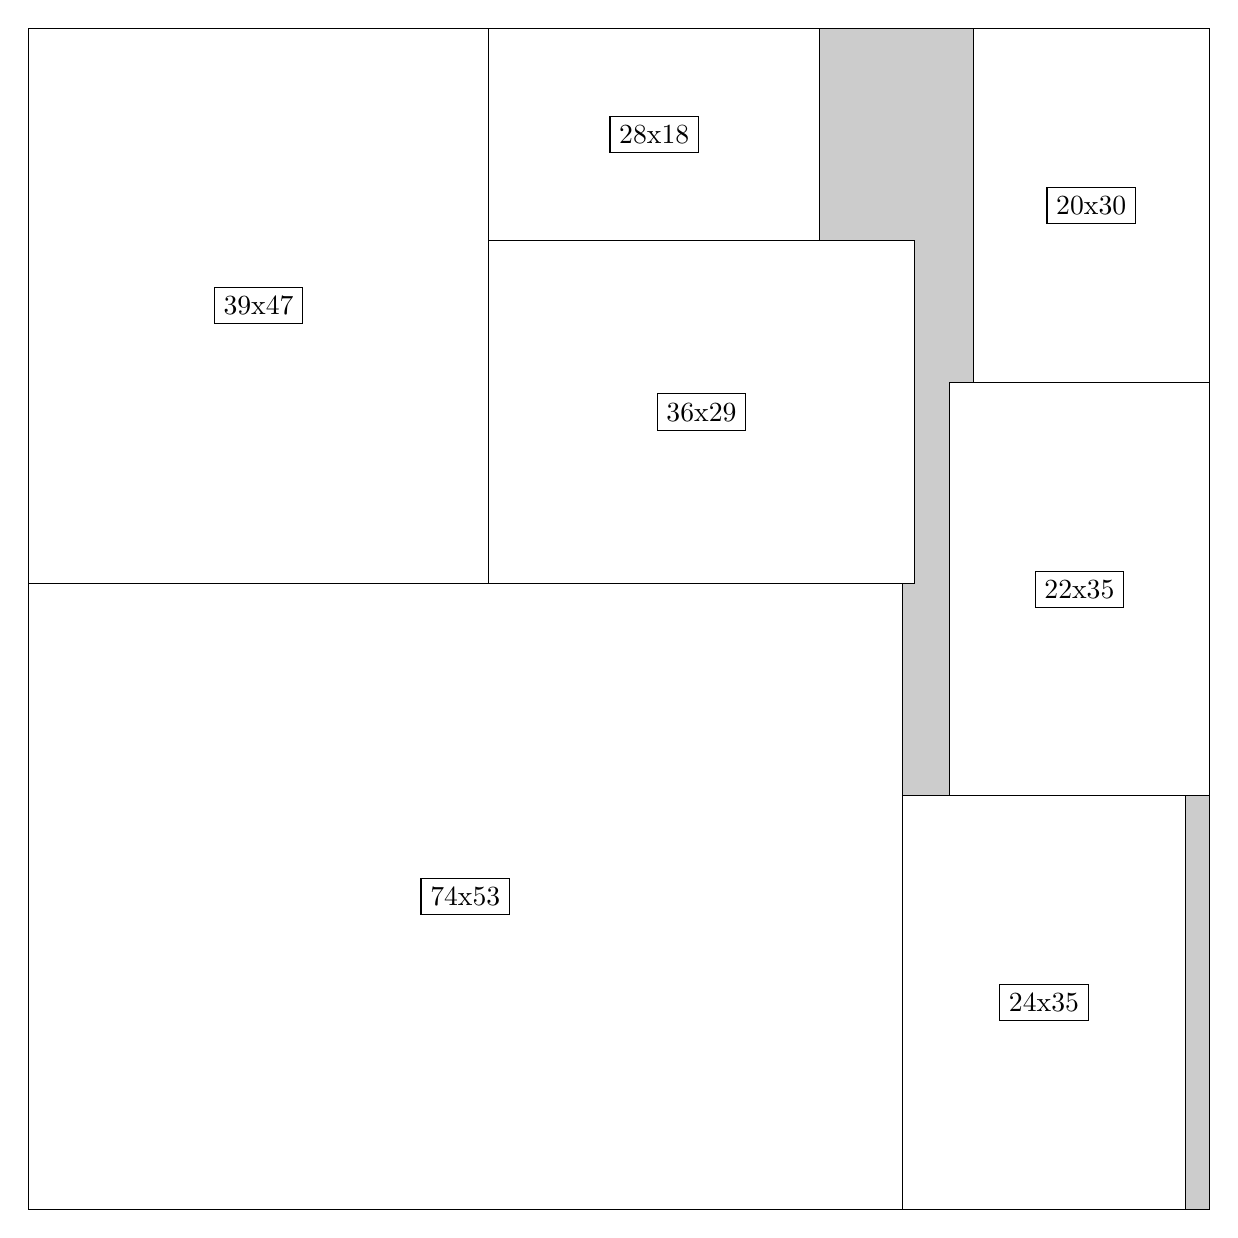
\begin{tikzpicture}[shorten >=1pt,scale=1.0,every node/.style={scale=1.0},->]
\tikzstyle{vertex}=[circle,fill=black!25,minimum size=14pt,inner sep=0pt]
\filldraw[fill=gray!40!white, draw=black] (0,0) rectangle (15.0,15.0);
\foreach \name/\x/\y/\w/\h in {74x53/0.0/0.0/11.1/7.949999999999999,39x47/0.0/7.949999999999999/5.85/7.05,22x35/11.7/5.25/3.3/5.25,36x29/5.85/7.949999999999999/5.3999999999999995/4.35,24x35/11.1/0.0/3.5999999999999996/5.25,20x30/12.0/10.5/3.0/4.5,28x18/5.85/12.299999999999999/4.2/2.6999999999999997}
\filldraw[fill=white!40!white, draw=black] (\x,\y) rectangle node[draw] (\name) {\name} ++(\w,\h);
\end{tikzpicture}


w =74 , h =53 , x =0 , y =0 , v =3922
\par
w =39 , h =47 , x =0 , y =53 , v =1833
\par
w =22 , h =35 , x =78 , y =35 , v =770
\par
w =36 , h =29 , x =39 , y =53 , v =1044
\par
w =24 , h =35 , x =74 , y =0 , v =840
\par
w =20 , h =30 , x =80 , y =70 , v =600
\par
w =28 , h =18 , x =39 , y =82 , v =504
\par
\newpage


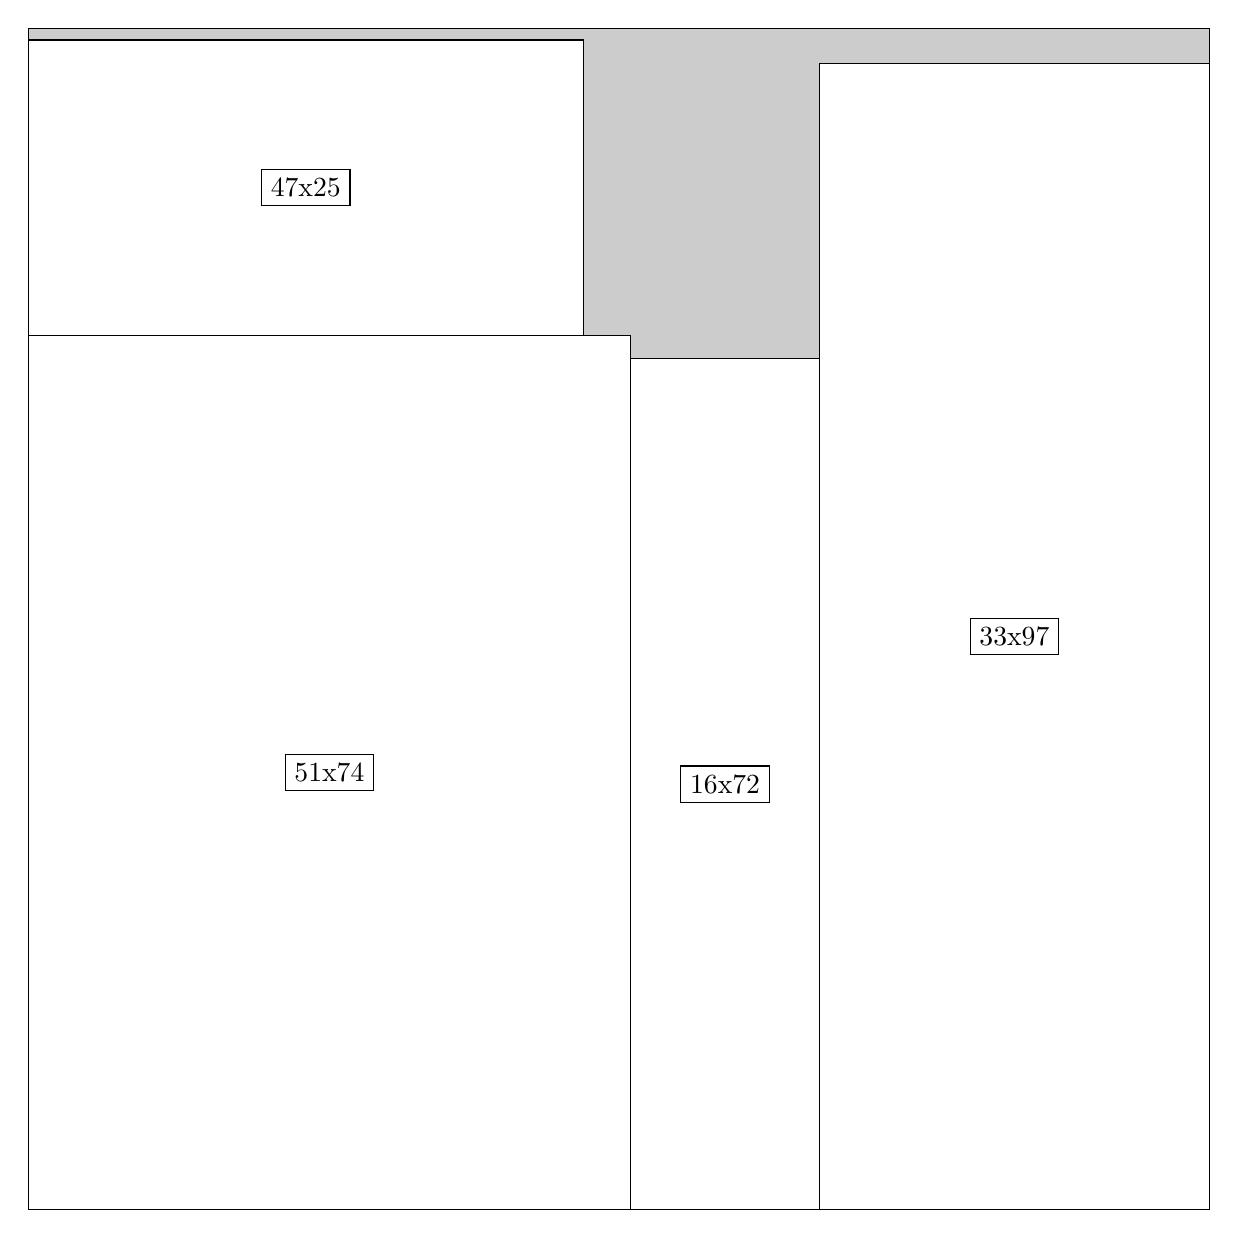
\begin{tikzpicture}[shorten >=1pt,scale=1.0,every node/.style={scale=1.0},->]
\tikzstyle{vertex}=[circle,fill=black!25,minimum size=14pt,inner sep=0pt]
\filldraw[fill=gray!40!white, draw=black] (0,0) rectangle (15.0,15.0);
\foreach \name/\x/\y/\w/\h in {33x97/10.049999999999999/0.0/4.95/14.549999999999999,47x25/0.0/11.1/7.05/3.75,16x72/7.6499999999999995/0.0/2.4/10.799999999999999,51x74/0.0/0.0/7.6499999999999995/11.1}
\filldraw[fill=white!40!white, draw=black] (\x,\y) rectangle node[draw] (\name) {\name} ++(\w,\h);
\end{tikzpicture}


w =33 , h =97 , x =67 , y =0 , v =3201
\par
w =47 , h =25 , x =0 , y =74 , v =1175
\par
w =16 , h =72 , x =51 , y =0 , v =1152
\par
w =51 , h =74 , x =0 , y =0 , v =3774
\par
\newpage


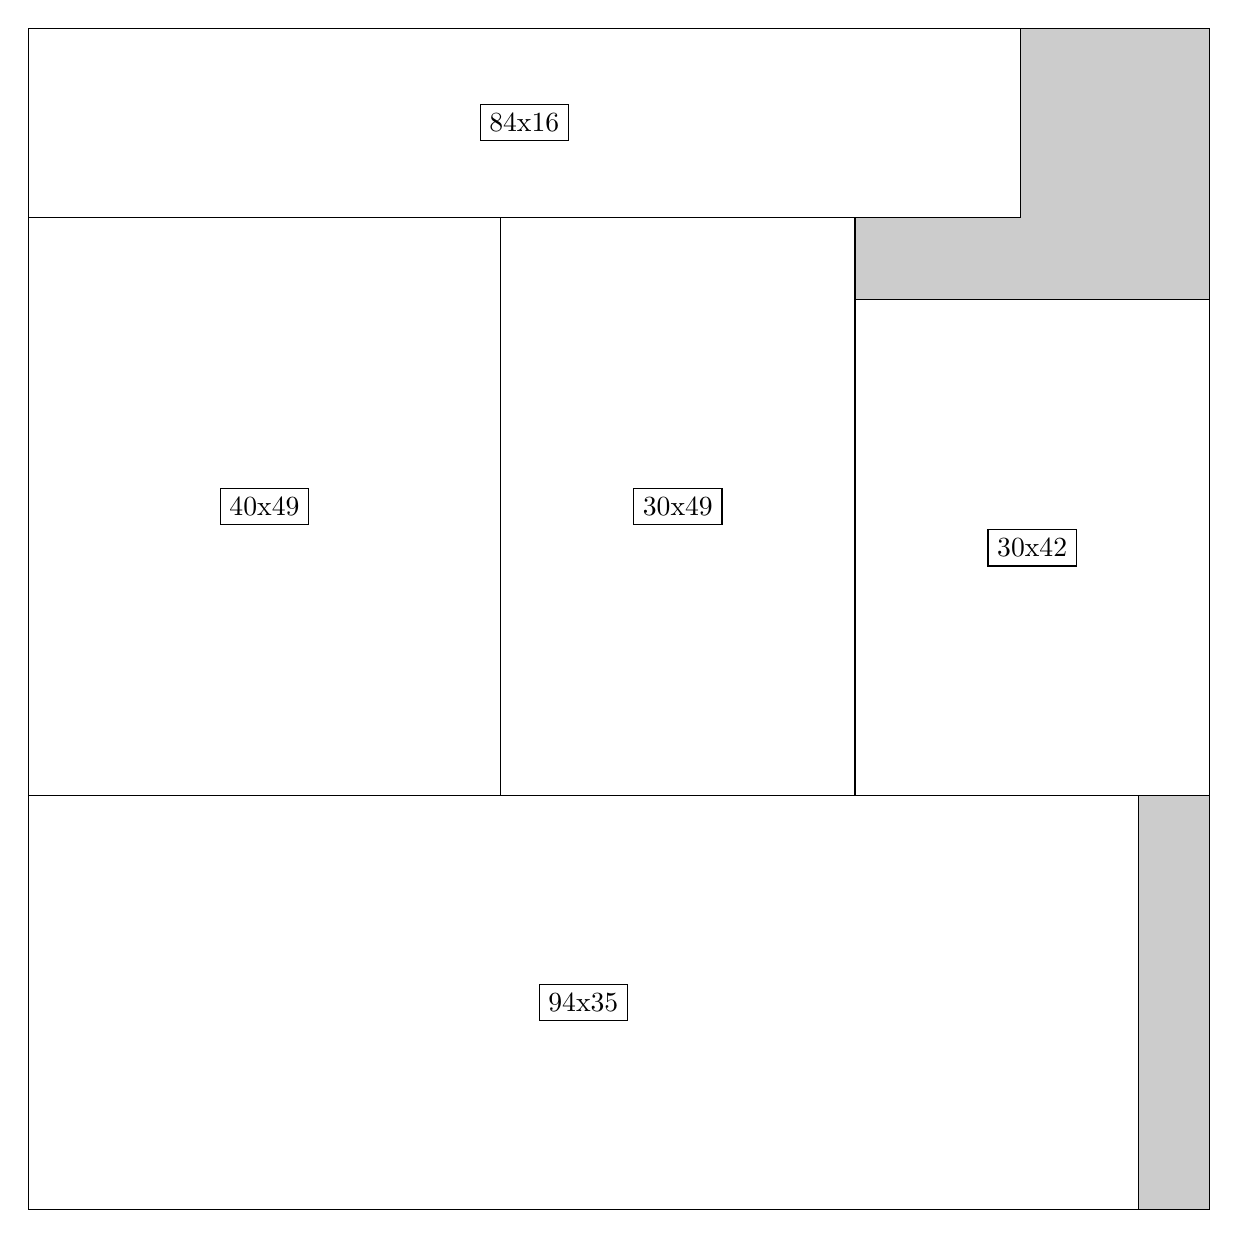
\begin{tikzpicture}[shorten >=1pt,scale=1.0,every node/.style={scale=1.0},->]
\tikzstyle{vertex}=[circle,fill=black!25,minimum size=14pt,inner sep=0pt]
\filldraw[fill=gray!40!white, draw=black] (0,0) rectangle (15.0,15.0);
\foreach \name/\x/\y/\w/\h in {94x35/0.0/0.0/14.1/5.25,40x49/0.0/5.25/6.0/7.35,30x49/6.0/5.25/4.5/7.35,84x16/0.0/12.6/12.6/2.4,30x42/10.5/5.25/4.5/6.3}
\filldraw[fill=white!40!white, draw=black] (\x,\y) rectangle node[draw] (\name) {\name} ++(\w,\h);
\end{tikzpicture}


w =94 , h =35 , x =0 , y =0 , v =3290
\par
w =40 , h =49 , x =0 , y =35 , v =1960
\par
w =30 , h =49 , x =40 , y =35 , v =1470
\par
w =84 , h =16 , x =0 , y =84 , v =1344
\par
w =30 , h =42 , x =70 , y =35 , v =1260
\par
\newpage


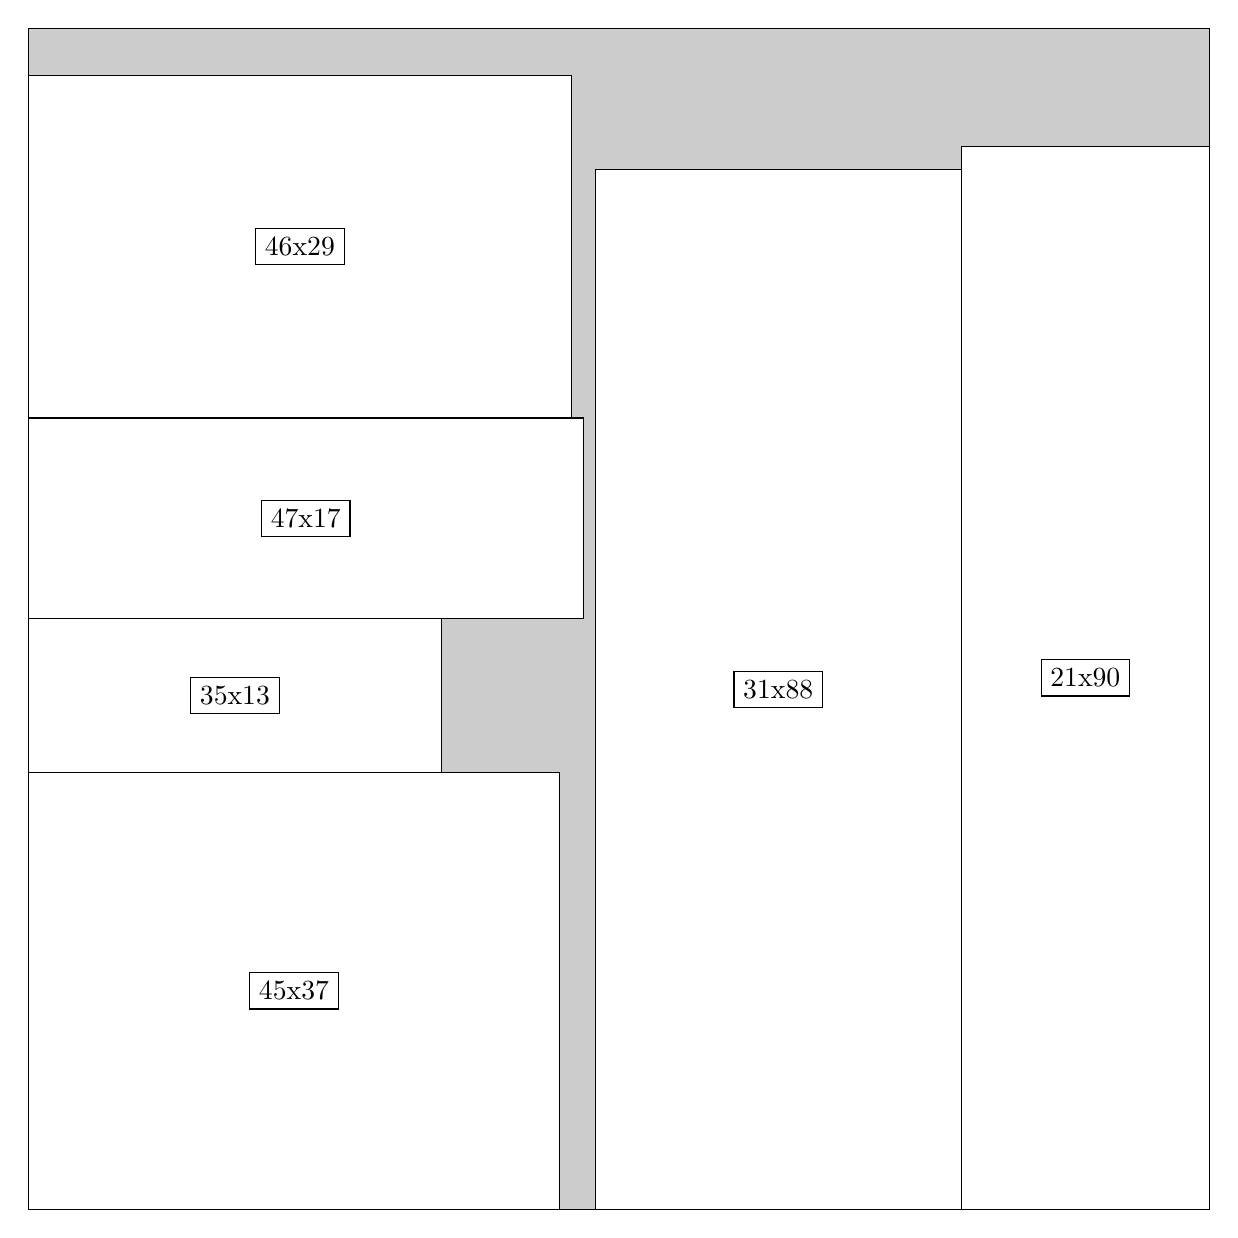
\begin{tikzpicture}[shorten >=1pt,scale=1.0,every node/.style={scale=1.0},->]
\tikzstyle{vertex}=[circle,fill=black!25,minimum size=14pt,inner sep=0pt]
\filldraw[fill=gray!40!white, draw=black] (0,0) rectangle (15.0,15.0);
\foreach \name/\x/\y/\w/\h in {31x88/7.199999999999999/0.0/4.6499999999999995/13.2,21x90/11.85/0.0/3.15/13.5,45x37/0.0/0.0/6.75/5.55,47x17/0.0/7.5/7.05/2.55,46x29/0.0/10.049999999999999/6.8999999999999995/4.35,35x13/0.0/5.55/5.25/1.95}
\filldraw[fill=white!40!white, draw=black] (\x,\y) rectangle node[draw] (\name) {\name} ++(\w,\h);
\end{tikzpicture}


w =31 , h =88 , x =48 , y =0 , v =2728
\par
w =21 , h =90 , x =79 , y =0 , v =1890
\par
w =45 , h =37 , x =0 , y =0 , v =1665
\par
w =47 , h =17 , x =0 , y =50 , v =799
\par
w =46 , h =29 , x =0 , y =67 , v =1334
\par
w =35 , h =13 , x =0 , y =37 , v =455
\par
\newpage


\end{document}